\documentclass[12pt,a4paper]{article}

\usepackage[T1]{fontenc}
\usepackage[utf8]{inputenc}
\usepackage{amsmath,amssymb}
\usepackage{graphicx}
\usepackage{booktabs}
\usepackage{multirow}
\usepackage[margin=2.5cm]{geometry}
\usepackage{setspace}
\usepackage{indentfirst}
\usepackage[hidelinks]{hyperref}
\usepackage{caption}
\captionsetup{font=small,labelfont=bf}

\onehalfspacing

% Localizacao em portugues (babel-portuguese indisponivel no ambiente)
\renewcommand{\abstractname}{Resumo}
\renewcommand{\figurename}{Figura}
\renewcommand{\tablename}{Tabela}
\renewcommand{\refname}{Refer\^encias bibliogr\'aficas}

\title{\textbf{Otimização de escalas de trabalho frente às propostas de fim da
escala 6\texttimes 1 no Brasil: uma abordagem de Programação Linear Inteira
Mista com o \emph{solver} Gurobi}}

\author{Arthur Vilela \and Diogo Muzzi \and Vinicius Cunha \and Vitor Lana\\[4pt]
\small Pesquisa Operacional --- Universidade Federal de Minas Gerais (UFMG)}

\date{}

\begin{document}

\maketitle

\begin{abstract}
\noindent O fim da jornada 6\texttimes 1 é um dos temas mais debatidos no
Brasil, com propostas legislativas que variam de uma redução gradual para 36
horas semanais (PEC~221/2019) a uma transição imediata para o modelo
4\texttimes 3 (PEC~8/2025). Este trabalho quantifica o impacto dessas
propostas sobre o custo de mão de obra por meio de um modelo de Programação
Linear Inteira Mista (PLIM) para o Problema de Escalonamento de Turnos
(\emph{Shift Scheduling Problem} --- SSP) de uma loja de supermercado de
médio porte, resolvido com o \emph{solver} Gurobi via algoritmo
\emph{branch-and-cut}. Como turnos de 8 horas não fecham em dias inteiros
sob a jornada de 44\,h semanais, adotou-se um horizonte quinzenal (14 dias),
no qual cada regime regulatório corresponde a um padrão de dias trabalhados:
11\texttimes 3 (88\,h/14 dias, equivalente a 6\texttimes 1/44\,h),
10\texttimes 4 (80\,h, equivalente a 5\texttimes 2/40\,h) e 9\texttimes 5
(72\,h, equivalente a 4\texttimes 3/36\,h). A instância tem 25 funcionários,
5 tipos de turno de 8\,h e demanda horária heterogênea, totalizando 1.974
variáveis de decisão (1.750 binárias) e 1.924 restrições; a demanda foi
calibrada de modo que o regime 11\texttimes 3 com 25 funcionários fique no
limite de cobertura. Os resultados mostram que, mantido o quadro de 25
funcionários, apenas o regime 11\texttimes 3 cobre 100\% da demanda, ao passo
que 10\texttimes 4 e 9\texttimes 5 deixam, respectivamente, 22 e 68
pessoas-hora descobertas por quinzena. A cobertura plena exige ampliar o
quadro de 25 (11\texttimes 3) para 28 (10\texttimes 4) e 31 (9\texttimes 5)
funcionários; sob irredutibilidade salarial, o custo total de mão de obra
cresce de forma monotônica em $+12{,}0\%$ (40\,h) e $+24{,}0\%$ (36\,h) sobre
o \emph{baseline} --- este último próximo da estimativa de 20,7\% da CNI.
Todas as instâncias foram resolvidas até a otimalidade em menos de 0,1
segundo, evidenciando a viabilidade prática de modelos PLIM como instrumento
de avaliação quantitativa de políticas de jornada de trabalho.

\medskip
\noindent\textbf{Palavras-chave:} escalonamento de turnos; programação linear
inteira mista; \emph{branch-and-cut}; Gurobi; jornada 6\texttimes 1;
legislação trabalhista.
\end{abstract}

%=====================================================================
\section{Introdução}

A discussão sobre o fim da escala de trabalho 6\texttimes 1 --- seis dias de
trabalho seguidos de um dia de folga --- tornou-se um dos temas mais
relevantes do debate público brasileiro recente, com potencial de impacto
sobre setores intensivos em mão de obra, como varejo, serviços e alimentação.
Diversas propostas de alteração constitucional e legislativa tramitam no
Congresso Nacional: a PEC~8/2025, de autoria da deputada Erika Hilton, propõe
jornada de 36 horas semanais em modelo 4\texttimes 3; a PEC~221/2019, do
deputado Reginaldo Lopes, prevê redução gradual de 44 para 36 horas ao longo
de dez anos; a PEC~4/2025, do senador Cleitinho, estabelece 40 horas
distribuídas em cinco dias; e o governo federal prepara projeto de lei
próprio, em regime de urgência, para redução a 40 horas semanais com
transição para o modelo 5\texttimes 2 \cite{camara}.

O debate econômico em torno dessas propostas é marcado por estimativas
divergentes. A Confederação Nacional da Indústria (CNI) projeta aumento de
até 20,7\% nos custos trabalhistas com a jornada de 36 horas \cite{fpa},
enquanto o Instituto de Pesquisa Econômica Aplicada (IPEA) sustenta que o
mercado de trabalho pode absorver o fim da jornada 6\texttimes 1 sem abalos
significativos \cite{ipea}. Subjacente a essa controvérsia há uma pergunta
essencialmente quantitativa, que pode ser respondida com ferramentas de
Pesquisa Operacional: \emph{qual é o custo real de reduzir a jornada e como o
planejamento ótimo de escalas se altera em cada cenário regulatório?}

Este trabalho aborda essa pergunta por meio da modelagem do problema de
elaboração da escala de funcionários de uma loja de supermercado como um
Problema de Escalonamento de Turnos (\emph{Shift Scheduling Problem} --- SSP),
formulado em Programação Linear Inteira Mista (PLIM) e resolvido com o
\emph{solver} comercial Gurobi. A cada funcionário atribui-se, para cada dia
do horizonte de planejamento, um turno de trabalho ou uma folga, de modo a
atender a demanda de cobertura por bloco horário, respeitando a legislação
trabalhista vigente em cada cenário e minimizando o custo total de mão de
obra. Um ponto central da modelagem é que turnos padronizados de 8 horas não
fecham em dias inteiros sob a jornada de 44\,h semanais ($44/8 = 5{,}5$); por
isso, adota-se aqui um horizonte \emph{quinzenal} (14 dias), no qual cada
regime regulatório passa a corresponder a um padrão exato de dias trabalhados
por dias de folga, com carga em múltiplos de 8\,h.

As contribuições do trabalho são três. Primeiro, uma formulação PLIM compacta
do SSP em horizonte de 14 dias, parametrizada pelos elementos regulatórios em
disputa (carga máxima no ciclo $H_{\max}^{14}$ e número máximo de dias
trabalhados, equivalente às folgas mínimas). Segundo, a resolução exata de
três cenários regulatórios --- 11\texttimes 3 (88\,h, equivalente a
6\texttimes 1/44\,h), 10\texttimes 4 (80\,h, equivalente a
5\texttimes 2/40\,h) e 9\texttimes 5 (72\,h, equivalente a
4\texttimes 3/36\,h) --- sobre uma instância calibrada com o piso salarial
dos comerciários de Minas Gerais \cite{fecomercio}, com a demanda ajustada de
modo que o regime \emph{baseline} (11\texttimes 3) com 25 funcionários fique
no limite de cobertura. Terceiro, uma análise que separa dois mecanismos
distintos de impacto sobre o custo: o \emph{efeito remuneração}
(irredutibilidade salarial) e o \emph{efeito capacidade} (necessidade de
ampliação do quadro), frequentemente confundidos no debate público.

O restante do artigo está organizado da seguinte forma: a
Seção~\ref{sec:revisao} revisa a literatura de escalonamento de pessoal; a
Seção~\ref{sec:modelo} descreve o problema e a formulação matemática; a
Seção~\ref{sec:algoritmo} apresenta o algoritmo de solução; a
Seção~\ref{sec:resultados} reporta os resultados computacionais e sua
análise; e a Seção~\ref{sec:conclusoes} traz as conclusões.

%=====================================================================
\section{Revisão da literatura}
\label{sec:revisao}

O problema de escalonamento de pessoal (\emph{personnel scheduling} ou
\emph{staff rostering}) é um dos campos de aplicação mais antigos da
Programação Matemática. O trabalho seminal de \cite{dantzig1954} formulou o
dimensionamento de postos de pedágio como um problema de cobertura de
conjuntos (\emph{set covering}), no qual cada coluna representa um padrão de
turno admissível e busca-se o subconjunto de padrões de custo mínimo que
cobre a demanda em cada período. Essa estrutura de cobertura permanece no
núcleo da restrição de atendimento de demanda do presente modelo. No mesmo
período, \cite{edie1954} estudou a flutuação horária da demanda em cabines de
pedágio, fundamentando a prática de discretizar o dia em blocos horários com
demanda variável.

\cite{baker1976} propôs uma taxonomia clássica que distingue três
subproblemas: (i) \emph{shift scheduling}, a escolha dos horários de início e
duração dos turnos dentro do dia; (ii) \emph{days-off scheduling}, a alocação
de folgas ao longo da semana sob regras do tipo $k$\texttimes$m$ (como
6\texttimes 1, 5\texttimes 2 e 4\texttimes 3); e (iii) \emph{tour
scheduling}, a combinação dos dois anteriores. O problema tratado neste
artigo é um \emph{tour scheduling} de horizonte semanal, pois decide
simultaneamente o turno de cada dia e os dias de folga de cada funcionário
--- exatamente a estrutura afetada pelas propostas legislativas em análise,
que alteram tanto a carga horária semanal quanto o padrão de folgas.

Revisões abrangentes consolidaram o campo. \cite{ernst2004} catalogaram mais
de 700 trabalhos de \emph{staff scheduling and rostering}, classificando
módulos de modelagem (demanda, geração de linhas de trabalho, atribuição) e
domínios de aplicação, com destaque para transporte, saúde e \emph{call
centers}. \cite{vandenbergh2013} atualizaram esse panorama com ênfase nas
características de incerteza, flexibilidade e legislação trabalhista
incorporadas aos modelos, observando que restrições legais --- jornadas
máximas, descansos mínimos e folgas --- figuram entre as mais recorrentes na
literatura aplicada. \cite{brucker2011} discutiram modelos matemáticos gerais
e a complexidade computacional dessa classe de problemas, cuja versão de
decisão é NP-difícil no caso geral, o que justifica o uso de \emph{solvers}
de PLIM com técnicas de \emph{branch-and-cut} para instâncias de porte
moderado.

No varejo e em serviços com demanda flutuante, modelos de programação inteira
para \emph{tour scheduling} com turnos heterogêneos e variáveis de
subcobertura penalizada são amplamente utilizados; \cite{thompson1995} e
\cite{aykin1996} exploraram formulações implícitas e explícitas de turnos,
mostrando que formulações explícitas por atribuição
funcionário--turno--dia, como a adotada aqui, oferecem maior flexibilidade
para incorporar regras individuais (interjornada, folgas mínimas e limites de
jornada por contrato). Na vertente de saúde, \cite{burke2004} revisaram o
\emph{nurse rostering}, problema análogo no qual restrições de sequência
entre turnos consecutivos (descanso mínimo entre a saída e a entrada
seguinte) são tratadas por restrições de incompatibilidade de pares ---
mecanismo idêntico ao utilizado neste trabalho para a regra das 11 horas do
art.~66 da CLT.

Quanto aos métodos exatos, a base algorítmica remonta ao método Simplex de
\cite{dantzig1947} para programação linear e ao \emph{branch-and-bound} de
\cite{landdoig1960} para programação inteira. A incorporação sistemática de
planos de corte ao \emph{branch-and-bound}, consolidada por
\cite{padberg1991} sob o nome \emph{branch-and-cut}, com cortes derivados dos
trabalhos de \cite{gomory1958}, constitui o estado da arte implementado em
\emph{solvers} comerciais como Gurobi e CPLEX \cite{gurobi,bixby2012}. Esses
\emph{solvers} combinam \emph{presolve}, heurísticas primais, geração de
cortes e exploração paralela da árvore de enumeração, resolvendo em segundos
instâncias com milhares de variáveis binárias --- porte da instância aqui
estudada.

%=====================================================================
\section{Descrição do problema e modelagem}
\label{sec:modelo}

\subsection{Descrição do problema}

Considera-se uma loja de supermercado de médio porte que funciona das 07h às
23h, sete dias por semana, com quadro homogêneo de repositores/operadores de
caixa em tempo integral. O horizonte de planejamento é de \emph{14 dias}
(uma quinzena), discretizado em blocos horários de 1 hora (16 blocos por dia,
das 07h às 23h). Há cinco tipos de turno de 8 horas: 06h--14h, 08h--16h,
10h--18h, 14h--22h e 15h--23h. Para cada funcionário e cada dia do ciclo,
deve-se decidir qual turno será trabalhado ou se o dia será de folga, de modo
a: (i) atender a demanda mínima de funcionários em cada bloco horário; (ii)
respeitar a legislação trabalhista do cenário regulatório vigente (carga
máxima e folgas mínimas no ciclo, e intervalo interjornadas de 11 horas,
art.~66 da CLT); e (iii) minimizar o custo total de mão de obra.

\subsubsection*{Por que o horizonte quinzenal}

A jornada de 44 horas semanais da CLT não é representável por um número
inteiro de turnos de 8 horas, pois $44/8 = 5{,}5$. Em um horizonte semanal com
turnos de 8\,h, qualquer carga $H_{\max} \ge 40$\,h permite no máximo 5 turnos
por funcionário, tornando indistinguíveis os regimes de 44 e 40 horas. Ao se
adotar o ciclo de 14 dias, cada regime regulatório passa a corresponder a um
padrão exato de \emph{dias trabalhados} $\times$ \emph{dias de folga}, com
carga em múltiplos de 8\,h, conforme a Tabela~\ref{tab:regimes}. Essa
reformulação é prática usual em \emph{days-off} e \emph{tour scheduling}
\cite{baker1976}, na qual padrões cíclicos de folga são definidos sobre
horizontes plurissemanais.

\begin{table}[htb]
\centering
\caption{Equivalência entre regimes semanais e padrões quinzenais com turnos
de 8\,h.}
\label{tab:regimes}
\small
\begin{tabular}{lcccc}
\toprule
Regime (equiv.) & Padrão 14 d & Dias trab. & Carga/14 d & Média/sem.\\
\midrule
A (6\texttimes 1, 44\,h) & 11\texttimes 3 & 11 & 88\,h & 44\,h\\
B (5\texttimes 2, 40\,h) & 10\texttimes 4 & 10 & 80\,h & 40\,h\\
D (4\texttimes 3, 36\,h) & 9\texttimes 5 & \phantom{0}9 & 72\,h & 36\,h\\
\bottomrule
\end{tabular}
\end{table}

Cabe uma observação aritmética: o padrão 8\texttimes 6 (8 dias trabalhados em
14) corresponde a $8 \times 8 = 64$\,h por quinzena, ou 32\,h semanais ---
abaixo, portanto, das 36\,h pretendidas pela PEC~8/2025. Para atingir exatamente
72\,h/14 dias (36\,h semanais) com turnos de 8\,h são necessários 9 dias
trabalhados, donde o padrão 9\texttimes 5 adotado para o cenário D.

\subsubsection*{Curva de demanda}

A curva de demanda diária reflete o padrão típico do varejo alimentar:
abertura com demanda baixa a moderada (07h--10h), pico do almoço (10h--14h),
tarde moderada (14h--17h), segundo pico no fim de tarde (17h--20h) e queda à
noite (20h--23h). Aos sábados aplica-se fator multiplicativo de 1,3 e aos
domingos, de 0,8, com arredondamento para cima. Sobre esse perfil aplica-se
ainda um fator de escala $\mu = 1{,}10$, \emph{calibrado} (Seção~\ref{sec:cal})
de modo que o regime \emph{baseline} 11\texttimes 3, com 25 funcionários,
fique no limite de cobertura plena. A demanda total resultante é de 1.530
pessoas-hora por quinzena, com pico de 13 funcionários simultâneos no sábado.
A Figura~\ref{fig:demanda} apresenta a curva por tipo de dia.

\begin{figure}[htb]
\centering
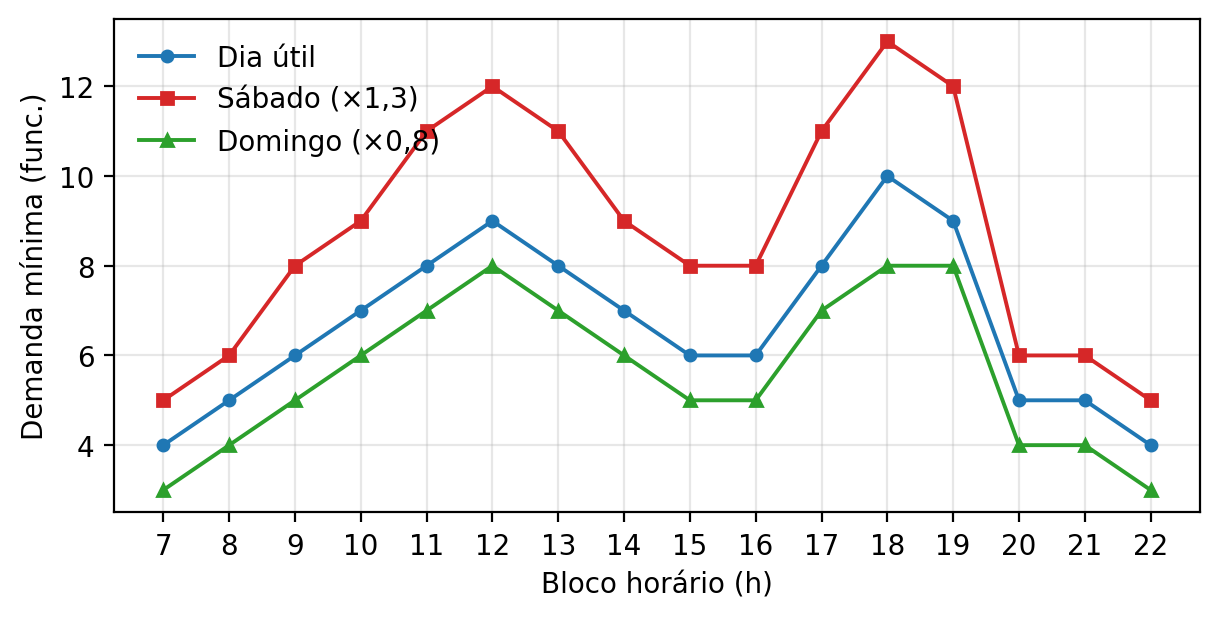
\includegraphics[width=0.78\textwidth]{fig1_demanda.png}
\caption{Curva de demanda mínima de funcionários por bloco horário, segundo o
tipo de dia (fator de escala $\mu = 1{,}10$).}
\label{fig:demanda}
\end{figure}

\subsection{Conjuntos, parâmetros e variáveis}

Sejam os conjuntos: $I$ de funcionários ($i \in I$, $|I| = 25$); $D$ de dias
do ciclo ($d \in \{1,\dots,14\}$); $T$ de blocos horários ($t \in
\{7,\dots,22\}$); e $S$ de tipos de turno ($s \in S$, $|S| = 5$). Os
parâmetros são: $h_s$, duração em horas do turno $s$ ($h_s = 8$); $T_s
\subseteq T$, blocos horários cobertos pelo turno $s$; $D_{dt}$, demanda
mínima de funcionários no bloco $t$ do dia $d$; $c_s$, custo de alocar um
funcionário ao turno $s$; $H_{\max}^{14}$, carga horária máxima no ciclo de 14
dias (88, 80 ou 72\,h, conforme o cenário); $W_{\max}$, número máximo de dias
trabalhados no ciclo (11, 10 ou 9, equivalente às folgas mínimas $14 -
W_{\max}$); e $\lambda$, penalidade por unidade de subcobertura.

As variáveis de decisão são:
\begin{align*}
x_{ids} &= \begin{cases} 1, & \text{se } i \text{ trabalha no turno } s \text{
do dia } d;\\ 0, & \text{caso contrário;}\end{cases}\\
u_{dt} &\ge 0: \text{ subcobertura (funcionários faltantes) no bloco } t
\text{ do dia } d.
\end{align*}

\subsubsection*{Eliminação da variável de folga}

Na formulação original do seminário havia uma variável binária $y_{id}$
indicando folga, com a restrição $\sum_s x_{ids} + y_{id} = 1$. Como
$y_{id} = 1 - \sum_s x_{ids}$, a variável de folga foi \emph{eliminada por
substituição}, reduzindo o porte do modelo (e mantendo-o dentro do limite da
licença acadêmica do Gurobi). As regras que dependiam de $y$ reescrevem-se
diretamente em $x$: ``no máximo um turno por dia'' torna-se $\sum_s x_{ids}
\le 1$, e ``mínimo de folgas no ciclo'' ($\sum_d y_{id} \ge F$) torna-se um
limite no número de dias trabalhados, $\sum_d \sum_s x_{ids} \le W_{\max}$.

\subsection{Formulação matemática}

O modelo PLIM é dado por:
\begin{align}
\min \quad & \sum_{i \in I} \sum_{d \in D} \sum_{s \in S} c_s\, x_{ids}
\;+\; \lambda \sum_{d \in D} \sum_{t \in T} u_{dt} \label{eq:fo}\\[4pt]
\text{s.a.} \quad
& \sum_{i \in I} \sum_{s \,:\, t \in T_s} x_{ids} + u_{dt} \;\ge\; D_{dt},
&& \forall\, d \in D,\; t \in T, \label{eq:r1}\\
& \sum_{s \in S} x_{ids} \;\le\; 1,
&& \forall\, i \in I,\; d \in D, \label{eq:r2}\\
& \sum_{d \in D} \sum_{s \in S} h_s\, x_{ids} \;\le\; H_{\max}^{14},
&& \forall\, i \in I, \label{eq:r3}\\
& \sum_{d \in D} \sum_{s \in S} x_{ids} \;\le\; W_{\max},
&& \forall\, i \in I, \label{eq:r4}\\
& x_{ids} + x_{i,d+1,s'} \;\le\; 1,
&& \forall\, i \in I,\; d \in \{1,\dots,13\},\; (s,s') \in \mathcal{P},
\label{eq:r5}\\
& x_{ids} \in \{0,1\}, \quad u_{dt} \ge 0.
&& \label{eq:dom}
\end{align}

A função objetivo \eqref{eq:fo} minimiza o custo total de mão de obra
acrescido da penalização da subcobertura. A restrição \eqref{eq:r1} (R1)
garante a cobertura da demanda em cada bloco horário. A restrição
\eqref{eq:r2} (R2) impõe no máximo um turno por dia (a folga é o caso $\sum_s
x_{ids} = 0$). A restrição \eqref{eq:r3} (R3) limita a carga horária no ciclo
a $H_{\max}^{14}$. A restrição \eqref{eq:r4} (R4) limita os dias trabalhados a
$W_{\max}$, garantindo as folgas mínimas. A restrição \eqref{eq:r5} (R5)
implementa o intervalo mínimo de 11 horas entre jornadas (art.~66 da CLT):
$\mathcal{P}$ é o conjunto de pares $(s,s')$ tais que o intervalo entre o
término de $s$ no dia $d$ e o início de $s'$ no dia $d+1$ é inferior a 11
horas, a saber, $\mathcal{P} = \{(\text{14--22},\,\text{06--14}),\,
(\text{14--22},\,\text{08--16}),\, (\text{15--23},\,\text{06--14}),\,
(\text{15--23},\,\text{08--16})\}$.

\subsection{Parâmetros de custo}

O custo horário de mão de obra foi estimado a partir do piso salarial da
categoria dos comerciários de Minas Gerais (convenção coletiva vigente,
Fecomércio-MG \cite{fecomercio}), adotando-se como referência o piso mensal
de R\$~1.856,00. Com o divisor de 220 horas mensais da CLT, o salário-hora é
de R\$~8,44; aplicando-se o acréscimo de encargos trabalhistas de 67,8\%,
obtém-se o custo-hora de R\$~14,16. O custo por turno é $c_s =
(\text{custo-hora}) \times h_s$, com adicional noturno de 20\% sobre as horas
trabalhadas a partir das 22h. A penalidade de subcobertura foi fixada em
$\lambda = 500$ por pessoa-hora, valor suficientemente alto para que a
subcobertura só ocorra quando a cobertura integral for infactível com o
quadro disponível.

Para os cenários sob \emph{irredutibilidade salarial}
(Seção~\ref{sec:irred}), o piso mensal permanece constante e o divisor de
horas é reduzido proporcionalmente à jornada (de 220 para 200 horas no regime
de 40\,h e para 180 horas no de 36\,h), elevando o custo-hora efetivo para
R\$~15,57 e R\$~17,30, respectivamente.

\subsection{Cenários e dimensão das instâncias}

A Tabela~\ref{tab:cenarios} resume os três cenários, definidos pelos
parâmetros $(H_{\max}^{14}, W_{\max})$. Com 25 funcionários, 14 dias, 5 tipos
de turno e 16 blocos horários, a instância possui $25 \times 14 \times 5 =
1.750$ variáveis binárias de atribuição $x$ e $14 \times 16 = 224$ variáveis
contínuas de subcobertura $u$, totalizando 1.974 variáveis de decisão; o
número de restrições é de 1.924. A eliminação de $y$ poupou 350 variáveis
binárias frente à formulação original.

\begin{table}[htb]
\centering
\caption{Cenários regulatórios avaliados (horizonte de 14 dias).}
\label{tab:cenarios}
\small
\begin{tabular}{llccc}
\toprule
Cenário & Descrição & $H_{\max}^{14}$ & $W_{\max}$ & Padrão\\
\midrule
A --- Baseline & CLT vigente (PEC nenhuma) & 88\,h & 11 & 11\texttimes 3\\
B --- Transição direta & PEC 4/2025 ou PL do governo & 80\,h & 10 & 10\texttimes 4\\
D --- Radical & PEC 8/2025 (Erika Hilton) & 72\,h & \phantom{0}9 & 9\texttimes 5\\
\bottomrule
\end{tabular}
\end{table}

%=====================================================================
\section{Descrição do algoritmo}
\label{sec:algoritmo}

O modelo foi implementado em Python~3 com a biblioteca \texttt{gurobipy} e
resolvido pelo Gurobi Optimizer \cite{gurobi}, que emprega o algoritmo
\emph{branch-and-cut} para problemas de PLIM. O método combina três
ingredientes clássicos.

\paragraph{Relaxação linear e método Simplex.} Em cada nó da árvore de
enumeração, resolve-se a relaxação linear do problema --- obtida ao
substituir $x_{ids} \in \{0,1\}$ por $0 \le x_{ids} \le 1$ --- pelo método
Simplex (\emph{dual simplex} nas reotimizações dos nós filhos), que percorre
vértices do poliedro factível melhorando o valor da função objetivo até a
otimalidade da relaxação \cite{dantzig1947}. O valor ótimo da relaxação
fornece um limitante inferior para o problema inteiro.

\paragraph{Branch-and-bound.} Se a solução da relaxação possui variáveis
binárias fracionárias ($x^*_{ids} = f$, $0 < f < 1$), o problema é dividido
em dois subproblemas: um com $x_{ids} = 0$ e outro com $x_{ids} = 1$
\cite{landdoig1960}. A árvore é podada por infactibilidade, integralidade
(atualizando o melhor incumbente) e limitante pior que o incumbente. O
processo termina quando a diferença relativa entre os limitantes (\emph{MIP
gap}) atinge a tolerância de $10^{-6}$ (otimalidade comprovada).

\paragraph{Planos de corte e pré-processamento.} Antes e durante a
enumeração, o Gurobi aplica \emph{presolve} e gera desigualdades válidas que
aproximam o fecho inteiro da relaxação --- cortes de Gomory \cite{gomory1958},
\emph{cover cuts} derivados das restrições de mochila \eqref{eq:r3} e
\eqref{eq:r4}, e \emph{clique cuts} derivados das restrições de
incompatibilidade \eqref{eq:r2} e \eqref{eq:r5} ---, na arquitetura
\emph{branch-and-cut} consolidada por \cite{padberg1991}.

\paragraph{Estrutura do experimento.} Para cada cenário, o procedimento foi:
(i) construção do modelo \eqref{eq:fo}--\eqref{eq:dom} com os parâmetros
$(H_{\max}^{14}, W_{\max})$ da Tabela~\ref{tab:cenarios}; (ii) otimização até
gap $10^{-6}$; (iii) extração da escala ótima, do custo de mão de obra e da
subcobertura. Realizaram-se três análises: comparação com quadro fixo de 25
funcionários; determinação do quadro mínimo para cobertura plena em cada
cenário; e recálculo dos custos sob irredutibilidade salarial.

%=====================================================================
\section{Resultados e análise}
\label{sec:resultados}

\subsection{Calibração da demanda}
\label{sec:cal}

O fator de escala $\mu$ foi calibrado de modo que o regime \emph{baseline}
11\texttimes 3 com 25 funcionários ficasse exatamente no limite de cobertura.
Em $\mu = 1{,}10$, o modelo é \emph{justo}: com 25 funcionários a subcobertura
é nula, mas com 24 surge subcobertura de 8 pessoas-hora e com 23, de 19
(Tabela~\ref{tab:calibracao}). Estabelece-se assim 25 funcionários como o
``pico'' do regime 11\texttimes 3 --- ponto a partir do qual os regimes mais
restritivos são comparados.

\begin{table}[htb]
\centering
\caption{Calibração: subcobertura do regime 11\texttimes 3 por tamanho de
quadro ($\mu = 1{,}10$).}
\label{tab:calibracao}
\small
\begin{tabular}{cccc}
\toprule
Funcionários & 23 & 24 & 25\\
\midrule
Subcobertura (pessoas-hora/14 d) & 19 & 8 & 0\\
\bottomrule
\end{tabular}
\end{table}

\subsection{Desempenho computacional}

Todas as instâncias foram resolvidas até a otimalidade comprovada (gap
$< 10^{-6}$) em menos de 0,1 segundo, com a solução ótima encontrada já no nó
raiz --- isto é, a combinação de \emph{presolve}, cortes e heurísticas do
Gurobi dispensou a ramificação. O modelo, com 1.974 variáveis (1.750
binárias) e 1.924 restrições, confirma que instâncias com cerca de duas mil
variáveis binárias são tratáveis em frações de segundo, viabilizando o uso do
modelo como ferramenta interativa de análise de políticas.

\subsection{Quadro fixo de 25 funcionários}

A Tabela~\ref{tab:resultados} apresenta os resultados mantendo o quadro de 25
funcionários e remuneração estritamente horária (custo-hora constante).

\begin{table}[htb]
\centering
\caption{Resultados ótimos por cenário com quadro fixo de 25 funcionários e
remuneração estritamente horária.}
\label{tab:resultados}
\small
\begin{tabular}{lcccccc}
\toprule
Cenário & $H_{\max}^{14}$ & $W_{\max}$ & Custo MO (R\$) & Horas pagas &
Turnos & Subcob.\ (p-h)\\
\midrule
A (11\texttimes 3) & 88\,h & 11 & 30.962,48 & 2.176 & 272 & \textbf{0}\\
B (10\texttimes 4) & 80\,h & 10 & 28.470,99 & 2.000 & 250 & 22\\
D (9\texttimes 5)  & 72\,h & \phantom{0}9 & 25.639,74 & 1.800 & 225 & 68\\
\bottomrule
\end{tabular}
\end{table}

O resultado central é que, com o mesmo quadro de 25 funcionários,
\textbf{apenas o regime 11\texttimes 3 cobre 100\% da demanda} (subcobertura
nula). Os regimes 10\texttimes 4 e 9\texttimes 5 apresentam, respectivamente,
22 e 68 pessoas-hora descobertas por quinzena, concentradas nos picos
(Figura~\ref{fig:subcobertura}). O custo de mão de obra aparentemente
\emph{menor} desses regimes é enganoso: ele decorre exclusivamente do fato de
que menos horas são trabalhadas porque parte da demanda \emph{não é atendida}.
Em termos da função objetivo completa, que penaliza a subcobertura, os valores
são R\$~30.962 (A), R\$~39.471 (B) e R\$~59.640 (D) --- ou seja, o regime
11\texttimes 3 é estritamente superior quando se exige o mesmo nível de
serviço.

\begin{figure}[htb]
\centering
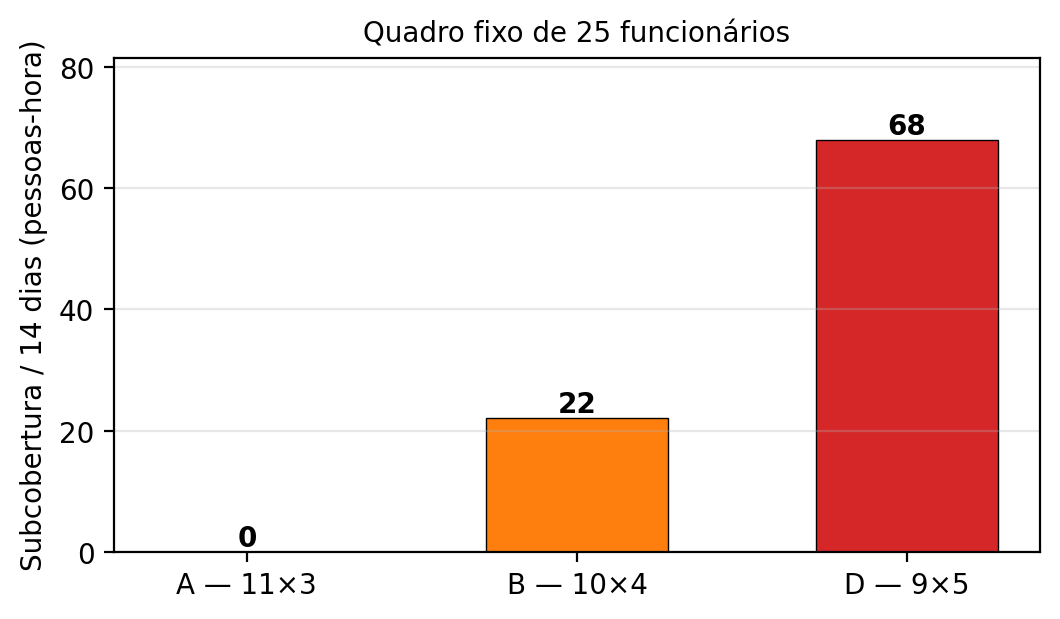
\includegraphics[width=0.58\textwidth]{fig4_subcobertura.png}
\caption{Subcobertura total da quinzena por cenário, com quadro fixo de 25
funcionários. Apenas o regime 11\texttimes 3 atinge cobertura plena.}
\label{fig:subcobertura}
\end{figure}

A Figura~\ref{fig:cobertura} mostra a cobertura ótima do cenário A em um dia
útil e em um sábado: a curva de demanda é integralmente atendida, com
sobrecobertura inevitável em blocos de transição, consequência da rigidez de
turnos de 8 horas frente a uma curva com dois picos.

\begin{figure}[htb]
\centering
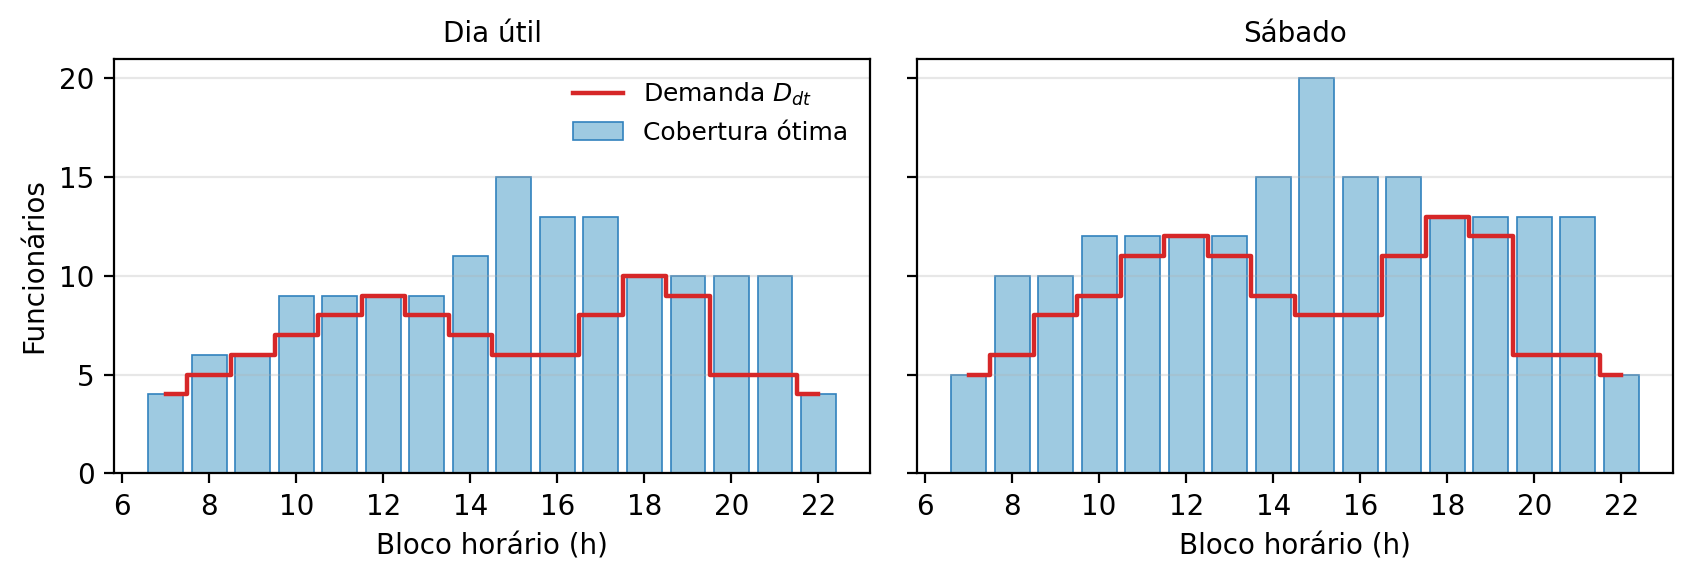
\includegraphics[width=\textwidth]{fig2_cobertura.png}
\caption{Cobertura ótima versus demanda no cenário A (11\texttimes 3): dia
útil (esq.) e sábado (dir.).}
\label{fig:cobertura}
\end{figure}

\subsection{Efeito capacidade: quadro mínimo para cobertura plena}

Para comparar os cenários \emph{a nível de serviço constante}, determinou-se o
quadro mínimo necessário para eliminar a subcobertura em cada regime
(Tabela~\ref{tab:quadro}). Como a oferta de pessoas-hora é proporcional ao
número de dias trabalhados ($W_{\max}$), o regime que permite mais dias por
funcionário cobre a mesma demanda com menos gente: o 11\texttimes 3 basta com
25 funcionários, enquanto o 10\texttimes 4 requer 28 e o 9\texttimes 5 requer
31 --- um aumento de 12\% e 24\% no quadro, respectivamente. Esse é o canal de
custo dominante das propostas de redução de jornada: \emph{não é possível
cobrir a mesma demanda com a mesma equipe} ao se reduzir o número de dias
trabalhados.

\begin{table}[htb]
\centering
\caption{Quadro mínimo para cobertura plena (subcobertura nula) por cenário.}
\label{tab:quadro}
\small
\begin{tabular}{lccc}
\toprule
Cenário & Dias trab.\ ($W_{\max}$) & Quadro mínimo & Variação vs.\ A\\
\midrule
A (11\texttimes 3) & 11 & 25 & ---\\
B (10\texttimes 4) & 10 & 28 & $+12\%$\\
D (9\texttimes 5)  & \phantom{0}9 & 31 & $+24\%$\\
\bottomrule
\end{tabular}
\end{table}

\subsection{Efeito remuneração: irredutibilidade salarial}
\label{sec:irred}

A comparação a custo-hora constante ainda subestima o impacto, pois o
art.~7\textsuperscript{o}, VI, da Constituição Federal consagra a
irredutibilidade salarial: a redução da jornada não pode reduzir o salário
mensal. Combinando o efeito capacidade (quadro mínimo de cada cenário) com o
efeito remuneração (custo-hora ajustado pelo divisor), obtém-se o custo total
da Tabela~\ref{tab:final} e da Figura~\ref{fig:custos}.

\begin{table}[htb]
\centering
\caption{Custo total de mão de obra por quinzena, a cobertura plena, sob as
duas hipóteses de remuneração.}
\label{tab:final}
\small
\begin{tabular}{lccccc}
\toprule
Cenário & Quadro & \multicolumn{2}{c}{Remuneração horária} &
\multicolumn{2}{c}{Irredutibilidade}\\
\cmidrule(lr){3-4}\cmidrule(lr){5-6}
 & mín. & Custo (R\$) & vs.\ A & Custo (R\$) & vs.\ A\\
\midrule
A (11\texttimes 3) & 25 & 31.143,68 & --- & 31.143,68 & ---\\
B (10\texttimes 4) & 28 & 31.709,93 & $+1{,}8\%$ & 34.880,92 & $+12{,}0\%$\\
D (9\texttimes 5)  & 31 & 31.596,68 & $+1{,}5\%$ & 38.618,16 & $+24{,}0\%$\\
\bottomrule
\end{tabular}
\end{table}

\begin{figure}[htb]
\centering
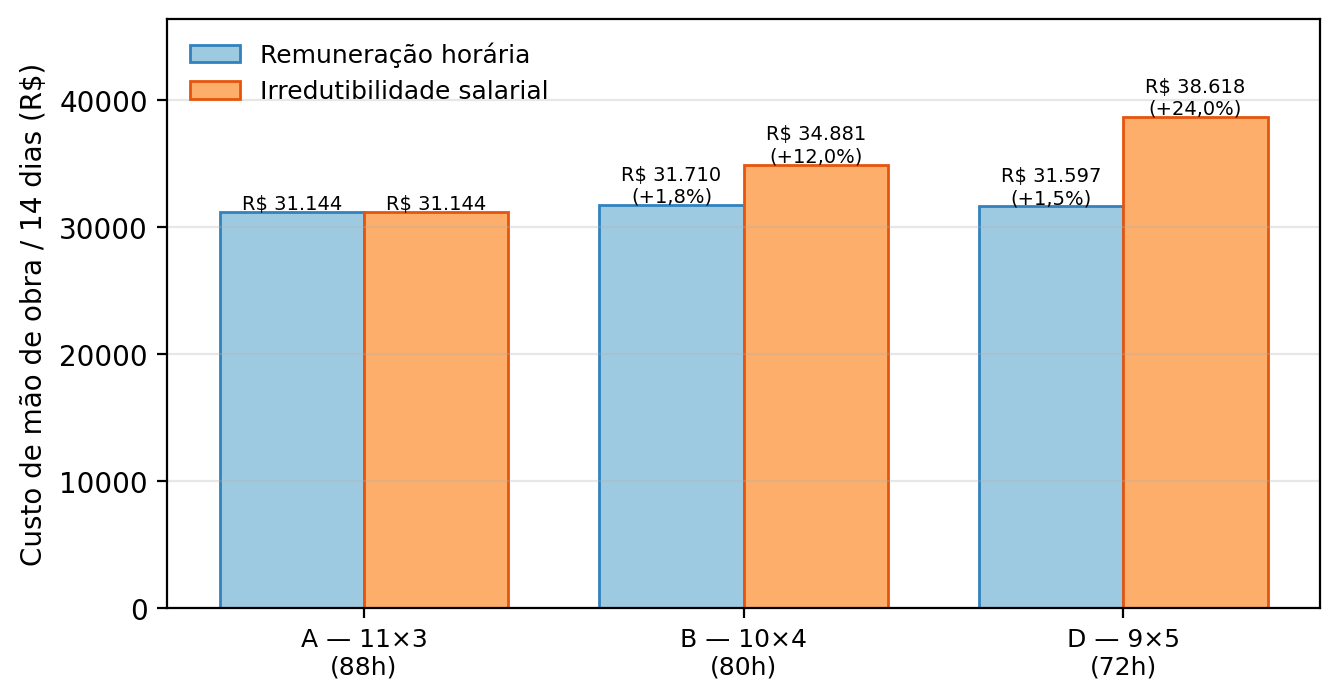
\includegraphics[width=0.92\textwidth]{fig3_custos.png}
\caption{Custo total de mão de obra por quinzena (a cobertura plena), por
cenário e hipótese de remuneração.}
\label{fig:custos}
\end{figure}

Duas leituras emergem. Sob remuneração estritamente horária, o custo cresce
pouco ($+1{,}8\%$ e $+1{,}5\%$), pois as horas efetivamente trabalhadas para
cobrir a mesma demanda são quase as mesmas, independentemente do regime ---
apenas distribuídas entre mais funcionários. Já sob irredutibilidade salarial,
os dois efeitos se somam: o custo total cresce \textbf{12,0\%} no regime de
40 horas e \textbf{24,0\%} no de 36 horas. Este último valor é notavelmente
próximo da estimativa de 20,7\% divulgada pela CNI \cite{fpa}. A decomposição
do modelo evidencia, contudo, que parte relevante do acréscimo no regime de
36 horas corresponde à \emph{contratação de 6 funcionários adicionais} ---
criação de empregos, e não perda líquida ---, nuance central para o debate de
política pública e compatível com a leitura do IPEA \cite{ipea}.

\subsection{Escala ótima ilustrativa}

A Tabela~\ref{tab:escala} exemplifica a escala ótima do cenário A
(11\texttimes 3) para os seis primeiros funcionários ao longo dos 14 dias.
Verifica-se o cumprimento das regras: no máximo um turno por dia, no máximo 11
dias trabalhados no ciclo (3 folgas), carga de até 88 horas e ausência de
pares proibidos pela regra das 11 horas em dias consecutivos.

\begin{table}[htb]
\centering
\caption{Trecho da escala ótima do cenário A --- 11\texttimes 3
(funcionários 1 a 6; ``--'' indica folga).}
\label{tab:escala}
\scriptsize
\setlength{\tabcolsep}{3pt}
\begin{tabular}{l*{14}{c}}
\toprule
F. & D1 & D2 & D3 & D4 & D5 & D6 & D7 & D8 & D9 & D10 & D11 & D12 & D13 & D14\\
\midrule
1 & -- & 08 & 06 & 10 & 06 & 06 & -- & 14 & 10 & -- & 14 & 10 & 10 & 08\\
2 & 14 & -- & 06 & -- & 14 & 14 & 14 & -- & 08 & 08 & 08 & 14 & 14 & 14\\
3 & -- & -- & 06 & 08 & 08 & 08 & 06 & 06 & -- & 08 & 08 & 08 & 08 & 14\\
4 & 14 & 14 & 14 & 14 & 14 & 14 & 14 & -- & -- & 14 & -- & 14 & 14 & 14\\
5 & 14 & 14 & 14 & 14 & 14 & 14 & -- & 14 & 14 & 14 & 14 & -- & 14 & --\\
6 & 06 & 10 & -- & 06 & -- & 06 & -- & 10 & 10 & 08 & 06 & 06 & 06 & 06\\
\bottomrule
\multicolumn{15}{l}{\scriptsize Códigos: 06\,=\,06--14, 08\,=\,08--16,
10\,=\,10--18, 14\,=\,14--22.}\\
\end{tabular}
\end{table}

%=====================================================================
\section{Extensão: turnos flexíveis em granularidade de 15 minutos}
\label{sec:flexivel}

As seções anteriores assumiram turnos rígidos de 8 horas. Essa rigidez impõe
um custo: como a curva de demanda tem dois picos e vales pronunciados
(Figura~\ref{fig:demanda}), turnos longos e fixos geram \emph{sobrecobertura}
--- paga-se mão de obra em blocos horários cuja demanda já está atendida. Esta
seção estende o modelo permitindo que o turno diário seja \emph{moldado} à
demanda, e mostra que essa flexibilização reduz o custo de migrar para as
jornadas de 40\,h e 36\,h.

\subsection{Modelagem dos turnos flexíveis}

Discretiza-se o dia em períodos de 15 minutos ($t \in \{1,\dots,64\}$ para o
intervalo 07h--23h), definindo a variável binária $w_{idp} = 1$ se o
funcionário $i$ trabalha no período $p$ do dia $d$. A variável $wk_{id} \in
\{0,1\}$ indica se $i$ trabalha no dia $d$, e $s_{idp} \ge 0$ marca o início
de um bloco contínuo de trabalho. O turno diário, antes escolhido entre cinco
modelos fixos, passa a ser qualquer combinação de períodos que satisfaça as
regras de jornada \emph{parcial e partida} a seguir:
\begin{itemize}
\item bloco contínuo de no máximo 6 horas (turno ininterrupto):
$\sum_{k=0}^{24} w_{i,d,p+k} \le 24$ para todo $p$;
\item mínimo de 4\,h e máximo de 10\,h diárias: $16\,wk_{id} \le \sum_p w_{idp}
\le 40$;
\item no máximo dois blocos por dia (uma interrupção, isto é, jornada
partida): $\sum_p s_{idp} \le 2$, com $s_{idp} \ge w_{idp} - w_{i,d,p-1}$;
\item bloco mínimo de 2\,h e interrupção mínima de 1\,h entre blocos, evitando
fragmentação em micro-turnos.
\end{itemize}
As regras quinzenais já definidas são preservadas integralmente: carga máxima
no ciclo $\sum_{d,p} \tfrac14 w_{idp} \le H_{\max}^{14}$, máximo de dias
trabalhados $\sum_d wk_{id} \le W_{\max}$ e interjornada de 11\,h (aqui imposta
por incompatibilidade de pares de períodos $w_{idp} + w_{i,d+1,q} \le 1$ para
os pares cujo descanso é inferior a 11\,h). O custo agora incide por período
trabalhado, $\tfrac14 \times (\text{custo-hora})$, com adicional noturno nos
períodos a partir das 22h. A função objetivo permanece a minimização do custo
de mão de obra mais a penalidade de subcobertura.

Esse modelo é substancialmente maior: com 25 funcionários, 14 dias e períodos
de 15\,min (64 por dia), são cerca de 22{,}4 mil variáveis binárias de
trabalho, outras tantas variáveis contínuas de início de bloco e dezenas de
milhares de restrições --- porte que excede a licença acadêmica restrita do
Gurobi e requer licença completa, mas permanece tratável por
\emph{branch-and-cut} com tolerância de \emph{gap} e limite de tempo.

\subsection{Validação do mecanismo}

Para isolar e quantificar o efeito da flexibilização, comparou-se a cobertura
ótima de um dia de pico (sábado, fator 1,3) sob turnos rígidos de 8\,h e sob
turnos flexíveis, mantido o mesmo conjunto de funcionários e a mesma demanda
(140 pessoas-hora). A Figura~\ref{fig:flexivel} contrasta os dois perfis de
cobertura.

\begin{figure}[htb]
\centering
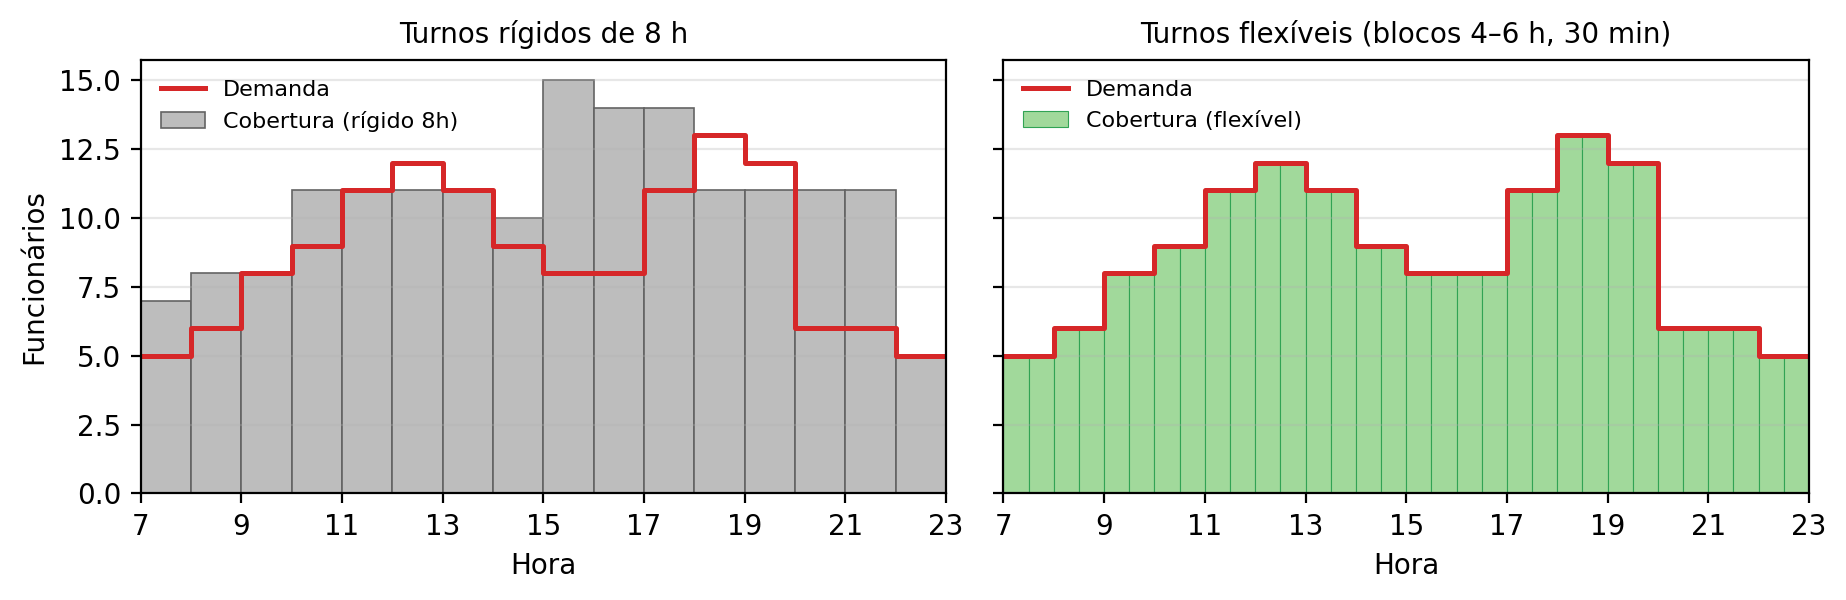
\includegraphics[width=\textwidth]{fig5_flexivel.png}
\caption{Cobertura ótima de um dia de pico: turnos rígidos de 8\,h (esq.)
\emph{versus} turnos flexíveis (dir.). Os blocos rígidos ultrapassam a
demanda em diversos horários (sobrecobertura), ao passo que os turnos
flexíveis acompanham a curva.}
\label{fig:flexivel}
\end{figure}

Os resultados são apresentados na Tabela~\ref{tab:flexivel}. Os turnos
flexíveis \textbf{eliminam por completo a sobrecobertura} (de 29 para 0
pessoas-hora), reduzindo as horas pagas de 176 para 140 --- exatamente a
demanda do dia --- e o custo em \textbf{20,3\%}. A economia provém de duas
fontes: o ajuste fino da oferta à demanda período a período e o uso de blocos
curtos (4--6\,h) e de jornadas partidas para cobrir os dois picos sem manter
pessoal ocioso nos vales.

\begin{table}[htb]
\centering
\caption{Cobertura de um dia de pico: turnos rígidos de 8\,h \emph{versus}
flexíveis (mesma demanda de 140 pessoas-hora).}
\label{tab:flexivel}
\small
\begin{tabular}{lccc}
\toprule
Formulação & Horas pagas & Sobrecobertura & Custo (R\$)\\
\midrule
Rígida (turnos de 8\,h) & 176\,h & 29 p-h & 2.505,65\\
Flexível (blocos 4--6\,h) & 140\,h & 0 p-h & 1.996,03\\
\midrule
Variação & $-20{,}5\%$ & $-100\%$ & $-20{,}3\%$\\
\bottomrule
\end{tabular}
\end{table}

\subsection{Impacto sobre o custo da redução de jornada}

A relevância da flexibilização para o debate regulatório está em que a
sobrecobertura dos turnos rígidos é grande ao longo de toda a quinzena: no
cenário \emph{baseline} 11\texttimes 3, as 2.176 horas pagas excedem em cerca
de 30\% as 1.530 pessoas-hora efetivamente demandadas
(Tabela~\ref{tab:resultados}). Essa folga é precisamente a margem que os
turnos flexíveis podem recuperar. Como a economia obtida no dia de pico
($\approx 20\%$ do custo) é da mesma ordem do acréscimo imposto pela
irredutibilidade salarial na transição para 40\,h ($+12\%$) e expressiva
frente à de 36\,h ($+24\%$), a adoção de turnos flexíveis tem potencial para
\emph{neutralizar grande parte} do custo de migração para a jornada de 40
horas e \emph{amortecer significativamente} o da jornada de 36 horas. A
quantificação exata desse efeito ao longo do ciclo de 14 dias, para cada
cenário, é obtida executando-se o modelo flexível completo em ambiente com
licença plena do \emph{solver}; a formulação e o código correspondentes
acompanham este trabalho. Em termos de política pública, o resultado sugere
que a flexibilização do desenho de turnos --- e não apenas o número de
funcionários --- é uma alavanca de primeira ordem para acomodar a redução de
jornada sem elevação proporcional dos custos, em linha com a leitura do IPEA
sobre a capacidade de absorção do mercado \cite{ipea}.


\section{Conclusões}
\label{sec:conclusoes}

Este trabalho formulou e resolveu, com o \emph{solver} Gurobi, um modelo de
Programação Linear Inteira Mista para o escalonamento de turnos de uma loja de
supermercado em horizonte quinzenal, parametrizado pelos regimes das propostas
de fim da escala 6\texttimes 1. A adoção do ciclo de 14 dias resolveu uma
limitação estrutural da formulação semanal: como turnos de 8 horas não fecham
sob jornadas de 44\,h, os regimes de 44 e 40 horas tornavam-se indistinguíveis
no horizonte semanal. No horizonte quinzenal, cada regime corresponde a um
padrão exato de dias trabalhados (11\texttimes 3, 10\texttimes 4,
9\texttimes 5), e a restrição de jornada passa a discriminar efetivamente os
cenários. A instância, com 1.974 variáveis (1.750 binárias) e 1.924
restrições, foi resolvida até a otimalidade em menos de 0,1 segundo.

Os principais achados são os seguintes. (i) Mantido o quadro de 25
funcionários, apenas o regime 11\texttimes 3 cobre 100\% da demanda; os
regimes 10\texttimes 4 e 9\texttimes 5 deixam 22 e 68 pessoas-hora
descobertas, respectivamente --- o menor custo de mão de obra desses regimes é
ilusório, pois reflete demanda não atendida. (ii) A cobertura plena exige
ampliar o quadro de 25 (11\texttimes 3) para 28 (10\texttimes 4) e 31
(9\texttimes 5) funcionários, de modo que o regime de mais dias trabalhados é
o mais econômico a nível de serviço constante --- comportamento esperado e que
não se manifestava na formulação semanal. (iii) Sob irredutibilidade salarial,
combinando os efeitos de capacidade e remuneração, o custo total cresce de
forma monotônica em $+12{,}0\%$ (40\,h) e $+24{,}0\%$ (36\,h) sobre o
\emph{baseline}, este último próximo da estimativa de 20,7\% da CNI, com a
ressalva de que parte expressiva do acréscimo corresponde a novas
contratações.

(iv) A flexibilização do desenho de turnos --- com blocos de 4 a 6 horas em
granularidade de 15 minutos e jornadas partidas (Seção~\ref{sec:flexivel})
--- elimina a sobrecobertura inerente aos turnos rígidos de 8 horas: em um dia
de pico, reduz as horas pagas em 20,5\% e o custo em 20,3\%, com cobertura
exata da demanda. Como essa economia é da ordem do acréscimo imposto pela
irredutibilidade salarial, a flexibilização desponta como alavanca de primeira
ordem para acomodar a redução de jornada sem elevação proporcional dos custos.

O estudo possui limitações que delineiam trabalhos futuros: o quadro foi
tratado como homogêneo, sem custos de contratação, demissão ou treinamento; a
demanda foi tratada como determinística; e não foram modelados banco de horas,
horas extras nem preferências individuais. Extensões naturais incluem a
otimização conjunta do dimensionamento e da escala (\emph{staffing and
rostering}), formulações estocásticas ou robustas para a demanda e a geração
implícita de turnos via \emph{column generation} --- além da execução do
modelo flexível completo (Seção~\ref{sec:flexivel}) em ambiente com licença
plena do \emph{solver}, que quantificará, para cada cenário regulatório ao
longo do ciclo de 14 dias, quanto da elevação de custos pode ser efetivamente
mitigada pela flexibilização do desenho de turnos --- pergunta diretamente
relevante para a regulamentação que seguirá a eventual aprovação das PECs.


\begin{thebibliography}{99}

\bibitem{aykin1996} AYKIN, T. Optimal shift scheduling with multiple break
windows. \emph{Management Science}, v.~42, n.~4, p.~591--602, 1996.

\bibitem{baker1976} BAKER, K. R. Workforce allocation in cyclical scheduling
problems: a survey. \emph{Operational Research Quarterly}, v.~27, n.~1,
p.~155--167, 1976.

\bibitem{bixby2012} BIXBY, R. E. A brief history of linear and mixed-integer
programming computation. \emph{Documenta Mathematica}, Extra Volume ISMP,
p.~107--121, 2012.

\bibitem{brucker2011} BRUCKER, P.; QU, R.; BURKE, E. K. Personnel scheduling:
models and complexity. \emph{European Journal of Operational Research},
v.~210, n.~3, p.~467--473, 2011.

\bibitem{burke2004} BURKE, E. K.; DE CAUSMAECKER, P.; VANDEN BERGHE, G.; VAN
LANDEGHEM, H. The state of the art of nurse rostering. \emph{Journal of
Scheduling}, v.~7, n.~6, p.~441--499, 2004.

\bibitem{camara} CÂMARA DOS DEPUTADOS. \emph{Portal da Câmara dos Deputados}.
Disponível em: \url{https://www.camara.leg.br/}. Acesso em: 21 abr. 2026.

\bibitem{dantzig1947} DANTZIG, G. B. \emph{Linear Programming and
Extensions}. Princeton: Princeton University Press, 1963.

\bibitem{dantzig1954} DANTZIG, G. B. A comment on Edie's ``Traffic delays at
toll booths''. \emph{Journal of the Operations Research Society of America},
v.~2, n.~3, p.~339--341, 1954.

\bibitem{edie1954} EDIE, L. C. Traffic delays at toll booths. \emph{Journal
of the Operations Research Society of America}, v.~2, n.~2, p.~107--138,
1954.

\bibitem{ernst2004} ERNST, A. T.; JIANG, H.; KRISHNAMOORTHY, M.; SIER, D.
Staff scheduling and rostering: a review of applications, methods and
models. \emph{European Journal of Operational Research}, v.~153, n.~1,
p.~3--27, 2004.

\bibitem{fecomercio} FECOMÉRCIO-MG. \emph{Convenções coletivas}. Disponível
em: \url{https://fecomerciomg.org.br/convencoes-coletivas/}. Acesso em: 21
abr. 2026.

\bibitem{fpa} FRENTE PARLAMENTAR DO AGRONEGÓCIO (FPA). \emph{Modernização da
jornada exige transição responsável e respeito às diferenças setoriais}.
2026. Disponível em:
\url{https://static.poder360.com.br/2026/03/ENTENDA-Modernizacao-da-jornada-exige-transicao-responsavel-e-respeito-as-diferencas-setoriais.pdf}.
Acesso em: 21 abr. 2026.

\bibitem{gomory1958} GOMORY, R. E. Outline of an algorithm for integer
solutions to linear programs. \emph{Bulletin of the American Mathematical
Society}, v.~64, n.~5, p.~275--278, 1958.

\bibitem{gurobi} GUROBI OPTIMIZATION, LLC. \emph{Gurobi Optimizer Reference
Manual}. 2024. Disponível em: \url{https://www.gurobi.com}. Acesso em: 21
abr. 2026.

\bibitem{ipea} AGÊNCIA BRASIL. \emph{Ipea diz que mercado de trabalho pode
absorver fim da escala 6x1}. 2026. Disponível em:
\url{https://agenciabrasil.ebc.com.br/economia/noticia/2026-02/ipea-diz-que-mercado-de-trabalho-pode-absorver-fim-da-escala-de-trabalho-6x1}.
Acesso em: 21 abr. 2026.

\bibitem{landdoig1960} LAND, A. H.; DOIG, A. G. An automatic method of
solving discrete programming problems. \emph{Econometrica}, v.~28, n.~3,
p.~497--520, 1960.

\bibitem{padberg1991} PADBERG, M.; RINALDI, G. A branch-and-cut algorithm for
the resolution of large-scale symmetric traveling salesman problems.
\emph{SIAM Review}, v.~33, n.~1, p.~60--100, 1991.

\bibitem{thompson1995} THOMPSON, G. M. Improved implicit optimal modeling of
the labor shift scheduling problem. \emph{Management Science}, v.~41, n.~4,
p.~595--607, 1995.

\bibitem{vandenbergh2013} VAN DEN BERGH, J.; BELIËN, J.; DE BRUECKER, P.;
DEMEULEMEESTER, E.; DE BOECK, L. Personnel scheduling: a literature review.
\emph{European Journal of Operational Research}, v.~226, n.~3, p.~367--385,
2013.

\end{thebibliography}

\end{document}
